\documentclass[tikz,border=6pt]{standalone}
% Shared preamble of the standalone figures: fonts as in the decks, the TikZ
% libraries, the notation, and the styles.
\usepackage[T1]{fontenc}
\usepackage[utf8]{inputenc}
\usepackage[sfdefault,lining]{FiraSans}
\usepackage{FiraMono}
\usepackage{amsmath}
\usetikzlibrary{positioning,arrows.meta,calc,shapes.misc,fit,backgrounds,
                decorations.pathreplacing,patterns,matrix}
% Notation for the MACE4D figures.
%
% Every parameter, symbol, default value, and constant that a figure shows is
% a macro here, so that the figures change from code names to symbols, or
% follow a change of a default, by editing this file alone.
%
%   \codenamestrue   renders each parameter as its code name (current setting)
%   \codenamesfalse  renders the symbolic form
%
% \sym{code name}{symbol} is the switch every parameter macro uses.  A
% parameter that exists on both models carries its owner in code mode.

\newif\ifcodenames
\codenamestrue

\providecommand{\code}[1]{\texttt{#1}}
\newcommand{\sym}[2]{\ifcodenames\code{#1}\else\ensuremath{#2}\fi}
\newcommand{\ctmodel}{\code{ct\_model}}
\newcommand{\macemodel}{\code{MACE4DModel}}
% A key line "code name <-> symbol", shown in code mode only.
\newcommand{\keyline}[2]{\ifcodenames#1~\ensuremath{\leftrightarrow}~\ensuremath{#2}\fi}

% ------------------------------------------------------------ math symbols
% These are always symbolic; the formulas use them, and the key lines tie
% them to the code names.
\newcommand{\symSigY}{\sigma_y}
\newcommand{\symSigProx}{\sigma_p}
\newcommand{\symSigNoise}{\sigma_n}
\newcommand{\symSigX}{\sigma_x}
\newcommand{\symSharpness}{s}
\newcommand{\symBeta}[1]{\beta_{#1}}
\newcommand{\symRho}{\rho}
\newcommand{\symNbrWeightTime}{b_t}
\newcommand{\symNumFrames}{T}
\newcommand{\symFramesPerRotation}{P}
\newcommand{\symOverlap}{f}

% ------------------------------------------------------------------ objects
\newcommand{\frameCube}[1]{\ensuremath{C_{#1}}}          % frame t of the 4D image
\newcommand{\fourD}{\ensuremath{x}}                      % the 4D image
\newcommand{\initImage}{\ensuremath{x^{0}}}              % the initial 4D image
\newcommand{\sinoFrame}[1]{\ensuremath{y_{#1}}}          % the views of frame t
\newcommand{\weightsFrame}[1]{\ensuremath{\Lambda_{#1}}} % the weights of frame t
\newcommand{\projFrame}[1]{\ensuremath{A_{#1}}}          % the frame model
\newcommand{\proxAgent}[1]{\ensuremath{F_{#1}}}          % the prox map of frame t
\newcommand{\dataFitAgent}{\ensuremath{F}}               % all frames' prox maps as one agent
\newcommand{\orientXY}{\sym{XY-t}{\mathrm{XY}t}}
\newcommand{\orientYZ}{\sym{YZ-t}{\mathrm{YZ}t}}
\newcommand{\orientXZ}{\sym{XZ-t}{\mathrm{XZ}t}}
\newcommand{\denoiser}[1]{\ensuremath{G_{#1}}}           % \denoiser{\orientXY}
\newcommand{\stateW}[1]{\ensuremath{W_{#1}}}             % the loop's input to agent k
\newcommand{\outX}[1]{\ensuremath{X_{#1}}}               % the output of agent k
\newcommand{\avgZ}{\ensuremath{z}}
\newcommand{\xbar}{\ensuremath{\bar{x}}}
\newcommand{\filterMatrix}{\sym{filter\_matrix}{H}}
\newcommand{\genInit}{\code{'init'}}                     % the generator of the partitions
\newcommand{\genIteration}{the iteration number}          % the generator of the subset order

% --------------------------------------------- parameters and their defaults
% Scan and frames (constructor arguments of MACE4DModel)
\newcommand{\pFramesPerRotation}{\sym{frames\_per\_rotation}{\symFramesPerRotation}}
\newcommand{\defFramesPerRotation}{6}
\newcommand{\pFrameOverlapFactor}{\sym{frame\_overlap\_factor}{\symOverlap}}
\newcommand{\defFrameOverlapFactor}{2.0}
\newcommand{\pNumFrames}{\sym{num\_frames}{\symNumFrames}}
\newcommand{\defNumFrames}{all}

% Set on ct_model; reach the frame models
\newcommand{\pSnrDb}{\sym{snr\_db}{\mathrm{SNR}_{\mathrm{dB}}}}
\newcommand{\defSnrDb}{30}
\newcommand{\pSharpnessCt}{\sym{ct\_model.sharpness}{\symSharpness_{\mathrm{ct}}}}
\newcommand{\defSharpnessCt}{1.0}
\newcommand{\pSigmaProxCt}{\sym{ct\_model.sigma\_prox}{\symSigProx^{\mathrm{ct}}}}
\newcommand{\pSigmaXCt}{\sym{ct\_model.sigma\_x}{\symSigX^{\mathrm{ct}}}}
\newcommand{\pPQTCt}{\sym{ct\_model.p, q, T}{(p, q, T)_{\mathrm{ct}}}}
\newcommand{\pSigmaY}{\sym{sigma\_y}{\symSigY}}

% Set on MACE4DModel
\newcommand{\pSigmaProxMace}{\sym{MACE4DModel.sigma\_prox}{\symSigProx}}
\newcommand{\defSigmaProxMace}{None (estimated per frame)}
\newcommand{\pSigmaNoise}{\sym{sigma\_noise}{\symSigNoise}}
\newcommand{\defSigmaNoise}{None (estimated)}
\newcommand{\pSigmaXMace}{\sym{MACE4DModel.sigma\_x}{\symSigX}}
\newcommand{\defSigmaXMace}{estimated}
\newcommand{\pSharpnessMace}{\sym{MACE4DModel.sharpness}{\symSharpness}}
\newcommand{\defSharpnessMace}{0.0}
\newcommand{\pPQTMace}{\sym{MACE4DModel.p, q, T}{(p, q, T)}}
\newcommand{\defPQT}{2.0, 1.2, 1.0}
\newcommand{\pNbrWeightTime}{\sym{nbr\_weight\_time}{\symNbrWeightTime}}
\newcommand{\defNbrWeightTime}{1.0}
\newcommand{\pMacePriorWeight}{\sym{mace\_prior\_weight}{\beta}}
\newcommand{\defMacePriorWeight}{0.5}
\newcommand{\pRhoMann}{\sym{rho\_mann}{\symRho}}
\newcommand{\defRhoMann}{0.5}
\newcommand{\pProxNumIterations}{\sym{prox\_num\_iterations}{N_p}}
\newcommand{\defProxNumIterations}{3}
\newcommand{\pProxPartitionAdvance}{\sym{prox\_partition\_advance}{a}}
\newcommand{\defProxPartitionAdvance}{1.0}
\newcommand{\pProxWarmStart}{\code{prox\_warm\_start}}
\newcommand{\defProxWarmStart}{True}
\newcommand{\pProxStopThreshold}{\code{prox\_stop\_threshold}}
\newcommand{\defProxStopThreshold}{0.02}
\newcommand{\pDenoiserWarmStart}{\code{denoiser\_warm\_start}}
\newcommand{\defDenoiserWarmStart}{False}
\newcommand{\pDenoiseSlabGb}{\code{denoise\_slab\_gb}}
\newcommand{\defDenoiseSlabGb}{2.0}
\newcommand{\pDejitter}{\code{dejitter}}
\newcommand{\defDejitter}{True}
\newcommand{\pDevicePool}{\code{set\_device\_pool}}
\newcommand{\pNumDevicesEnv}{\code{MBIRTORCH\_NUM\_DEVICES}}

% Arguments of MACE4DModel.recon
\newcommand{\pMaxIterations}{\sym{max\_iterations}{N}}
\newcommand{\defMaxIterations}{10}
\newcommand{\pStopThreshold}{\code{stop\_threshold\_change\_pct}}
\newcommand{\defStopThreshold}{0.2}
\newcommand{\pSeed}{\code{seed}}
\newcommand{\defSeed}{None}
\newcommand{\pInitRecon}{\code{init\_recon}}
\newcommand{\pInitDir}{\code{init\_dir}}

% ---------------------------------------------------------------- constants
\newcommand{\cInitIterations}{15}        % iterations of the per-frame initial image
\newcommand{\cDenoiseMaxIterations}{15}  % iterations per denoised volume, at most
\newcommand{\cDenoiseStopPct}{0.05}      % percent change that stops a denoised volume
\newcommand{\cSigmaXFactor}{0.2}         % sigma_x and sigma_prox estimates: factor * 2^sharpness * std
\newcommand{\cSigmaXFloor}{10^{-6}}      % floor of the denoiser sigma_x estimate
\newcommand{\cSigmaXBase}{1.0}           % base default of sigma_x when no estimate runs
\newcommand{\cDenoiseSubsets}{16}        % pixel subsets of a denoiser partition, at most
\newcommand{\cPixelsPerSubset}{64}       % fewer pixels per subset than this and the count drops

% ------------------------------------------- symbols the figures use inline
\newcommand{\symPriorWeight}{\ensuremath{w}}    % the value of the prior weight
\newcommand{\symFilterMatrix}{\ensuremath{H}}   % the temporal filter
\newcommand{\symFrameIndex}{\ensuremath{t}}
\newcommand{\symNumDevices}{\ensuremath{n}}     % the size of the device pool
\newcommand{\degsym}{\ensuremath{^{\circ}}}
% Argument values of the device pool selector
\newcommand{\valNone}{\code{None}}
\newcommand{\valCpu}{\code{'cpu'}}
\newcommand{\valGpu}{\code{'gpu'}}
% Derived defaults, in degrees (integers; add rounding if a default ever gives a fraction)
\newcommand{\defFrameStepDeg}{\pgfmathparse{int(360/\defFramesPerRotation)}\pgfmathresult}
\newcommand{\defFrameSpanDeg}{\pgfmathparse{int(\defFrameOverlapFactor*360/\defFramesPerRotation)}\pgfmathresult}
% Axis labels of the 4D image
\newcommand{\axisT}{\ensuremath{t}}
\newcommand{\axisX}{\ensuremath{x}}
\newcommand{\axisY}{\ensuremath{y}}
\newcommand{\axisZ}{\ensuremath{z}}

% Colors and TikZ styles shared by the MACE4D figures.
%
% Blue is the data-fit side, green the priors, amber the consensus state.
% A solid arrow carries a value the user set; a dashed arrow carries an
% estimate.  \cube draws one frame of the 4D image.

\definecolor{datafitBlue}{HTML}{3D6B99}
\definecolor{priorGreen}{HTML}{2E7D32}
\definecolor{stateAmber}{HTML}{B26B1F}
\definecolor{warnRed}{HTML}{A23B3B}
\definecolor{inkGray}{HTML}{5A5A5A}
\definecolor{lineGray}{HTML}{9A9A9A}
\definecolor{paleBlue}{HTML}{E3ECF5}
\definecolor{paleGreen}{HTML}{E4F0E4}
\definecolor{paleAmber}{HTML}{F5EBDD}
\definecolor{paleGray}{HTML}{F0F0F0}

\tikzset{
  every node/.style={font=\small},
  box/.style={draw, rounded corners=3pt, thick, align=center, inner sep=5pt,
              minimum height=8mm},
  datafit/.style={box, draw=datafitBlue, fill=paleBlue},
  prior/.style={box, draw=priorGreen, fill=paleGreen},
  state/.style={box, draw=stateAmber, fill=paleAmber},
  plain/.style={box, draw=lineGray, fill=paleGray},
  note/.style={font=\footnotesize, text=inkGray, align=left},
  notebox/.style={note, draw=lineGray, rounded corners=2pt, inner sep=4pt,
                  fill=white},
  param/.style={font=\footnotesize, align=left},
  title/.style={font=\bfseries, align=left},
  setarrow/.style={-{Stealth[length=2mm]}, thick},
  estarrow/.style={-{Stealth[length=2mm]}, thick, dashed, inkGray},
  flow/.style={-{Stealth[length=2mm]}, semithick},
  flowblue/.style={flow, datafitBlue},
  flowgreen/.style={flow, priorGreen},
  flowamber/.style={flow, stateAmber},
  cut/.style={-{Stealth[length=1.5mm]}, thin, inkGray},
  cubeFront/.style={fill=white, draw=black!70, thin},
  cubeTop/.style={fill=black!8, draw=black!70, thin},
  cubeSide/.style={fill=black!20, draw=black!70, thin},
}

% \cube{x}{y}{size}{label}: a cube whose front face has its lower left
% corner at (x, y) and side length size, with a label on the front face.
\newcommand{\cube}[4]{%
  \begin{scope}[shift={(#1,#2)}]
    \pgfmathsetmacro{\cubeDepth}{0.35*#3}
    \draw[cubeTop] (0,#3) -- (\cubeDepth,#3+\cubeDepth) -- (#3+\cubeDepth,#3+\cubeDepth) -- (#3,#3) -- cycle;
    \draw[cubeSide] (#3,0) -- (#3+\cubeDepth,\cubeDepth) -- (#3+\cubeDepth,#3+\cubeDepth) -- (#3,#3) -- cycle;
    \draw[cubeFront] (0,0) rectangle (#3,#3);
    \node at (0.5*#3,0.5*#3) {#4};
  \end{scope}}

% \arrowkey{x}{y}: the legend of the two arrow kinds, anchored at (x, y).
\newcommand{\arrowkey}[2]{%
  \draw[setarrow] (#1,#2) -- ++(1,0) node[note, right] {set by the user};
  \draw[estarrow] (#1,#2-0.45) -- ++(1,0) node[note, right] {estimated from the data};}



% Keep the words of the notes whole.
\hyphenpenalty=10000
\exhyphenpenalty=10000

\begin{document}
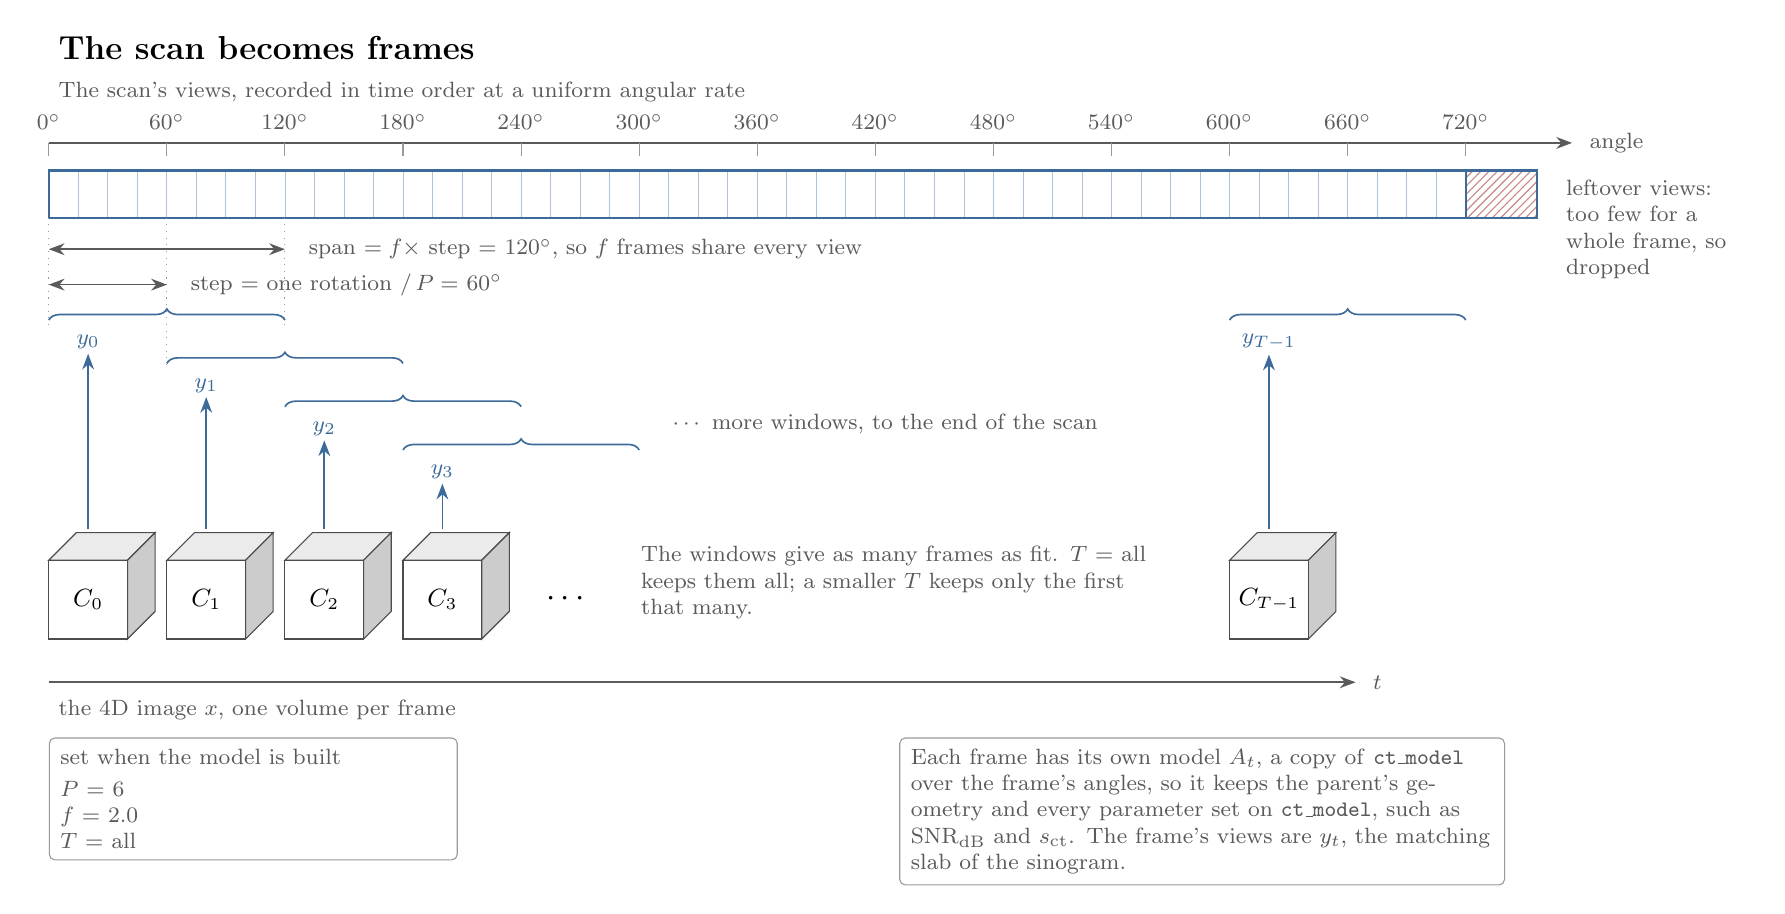
\begin{tikzpicture}

% Scale of the view strip and the landmarks along it.
\pgfmathsetmacro{\ds}{0.025}                              % cm per degree
\pgfmathsetmacro{\stepdeg}{360/\defFramesPerRotation}
\pgfmathsetmacro{\spandeg}{\defFrameOverlapFactor*\stepdeg}
\pgfmathsetmacro{\stepx}{\stepdeg*\ds}
\pgfmathsetmacro{\spanx}{\spandeg*\ds}
\pgfmathsetmacro{\nstep}{int(2*\defFramesPerRotation)}     % steps in the two rotations drawn
\pgfmathsetmacro{\xend}{\nstep*\stepx}
\pgfmathsetmacro{\xtail}{\xend+0.6*\stepx}
\pgfmathsetmacro{\xlast}{\xend-\spanx}                     % start of the last window
\pgfmathsetmacro{\nview}{int(4*\nstep)}                    % view marks drawn
\pgfmathsetmacro{\viewgap}{\stepx/4}

% Heights of the bands.
\def\ystripb{9.9}\def\ystript{10.5}\def\yaxis{10.85}
\def\yspan{9.5}\def\ystep{9.05}
\def\ybrone{8.6}\def\ydrop{0.55}
\def\ycube{4.55}\def\cubesize{1.0}\def\yarrow{5.95}
\def\ytime{4.0}\def\ybox{3.3}

% ------------------------------------------------------------------- title
\node[title, font=\large\bfseries, anchor=west] at (0,12.05) {The scan becomes frames};
\node[note, anchor=west] at (0,11.5)
  {The scan's views, recorded in time order at a uniform angular rate};

% -------------------------------------------------------------- angle axis
\draw[flow, inkGray] (0,\yaxis) -- (\xtail+0.45,\yaxis);
\node[note, anchor=west] at (\xtail+0.55,\yaxis) {angle};
\foreach \k in {0,...,\nstep}{
  \pgfmathsetmacro{\xt}{\k*\stepx}
  \pgfmathsetmacro{\dg}{int(\k*\stepdeg)}
  \draw[lineGray] (\xt,\yaxis) -- (\xt,\yaxis-0.16);
  \node[note, anchor=south] at (\xt,\yaxis+0.04) {\dg\degsym};}

% ------------------------------------------------ the strip of scan views
\fill[white] (0,\ystripb) rectangle (\xend,\ystript);
\foreach \i in {0,...,\nview}{
  \pgfmathsetmacro{\xv}{\i*\viewgap}
  \draw[datafitBlue!40, line width=0.3pt] (\xv,\ystripb) -- (\xv,\ystript);}
\draw[datafitBlue, thick] (0,\ystripb) rectangle (\xend,\ystript);
% the trailing views, too few for a whole frame
\fill[white] (\xend,\ystripb) rectangle (\xtail,\ystript);
\fill[pattern=north east lines, pattern color=warnRed!60]
  (\xend,\ystripb) rectangle (\xtail,\ystript);
\draw[datafitBlue, thick] (\xend,\ystripb) rectangle (\xtail,\ystript);
\node[note, anchor=north west, text width=2.3cm] at (\xtail+0.25,\ystript)
  {leftover views: too few for a whole frame, so dropped};

% --------------------------------------------- the step and span of a frame
\draw[lineGray, dotted] (0,\ystripb) -- (0,\ybrone-0.05);
\draw[lineGray, dotted] (\spanx,\ystripb) -- (\spanx,\ybrone-0.05);
\draw[lineGray, dotted] (\stepx,\ystripb) -- (\stepx,\ybrone-\ydrop-0.05);
\draw[flow, {Stealth[length=2mm]}-{Stealth[length=2mm]}, inkGray] (0,\yspan) -- (\spanx,\yspan);
\node[note, anchor=west] at (\spanx+0.18,\yspan)
  {span \ensuremath{=\symOverlap\times} step \ensuremath{=} \defFrameSpanDeg\degsym,
   so \ensuremath{\symOverlap} frames share every view};
\draw[flow, {Stealth[length=2mm]}-{Stealth[length=2mm]}, inkGray] (0,\ystep) -- (\stepx,\ystep);
\node[note, anchor=west] at (\stepx+0.18,\ystep)
  {step \ensuremath{=} one rotation \ensuremath{/\,\symFramesPerRotation=} \defFrameStepDeg\degsym};

% ----------------------------------------------- the window of each frame
\foreach \t in {0,...,3}{
  \pgfmathsetmacro{\xa}{\t*\stepx}
  \pgfmathsetmacro{\xb}{\xa+\spanx}
  \pgfmathsetmacro{\yb}{\ybrone-\t*\ydrop}
  \draw[decorate, decoration={brace, amplitude=4pt}, datafitBlue, semithick]
    (\xa,\yb) -- (\xb,\yb);
  \node[note, text=datafitBlue, inner sep=1.5pt] (win\t) at (\xa+0.5,\yb-0.28)
    {\sinoFrame{\t}};}
\draw[decorate, decoration={brace, amplitude=4pt}, datafitBlue, semithick]
  (\xlast,\ybrone) -- (\xend,\ybrone);
\node[note, text=datafitBlue, inner sep=1.5pt] (winlast) at (\xlast+0.5,\ybrone-0.28)
  {\sinoFrame{\symNumFrames-1}};
\node[note, anchor=west] at (\spanx+3*\stepx+0.3,\ybrone-2.4*\ydrop)
  {\ensuremath{\cdots} more windows, to the end of the scan};

% ------------------------------------------- the 4D image, one cube a frame
\foreach \t in {0,...,3}{
  \pgfmathsetmacro{\xc}{\t*\stepx}
  \cube{\xc}{\ycube}{\cubesize}{\frameCube{\t}}}
\cube{\xlast}{\ycube}{\cubesize}{\frameCube{\symNumFrames-1}}
\node[font=\large] at (4*\stepx+0.6,\ycube+0.5) {\ensuremath{\cdots}};
\foreach \t in {0,...,3}{
  \pgfmathsetmacro{\xc}{\t*\stepx+0.5}
  \draw[flowblue] (\xc,\yarrow) -- (win\t.south);}
\draw[flowblue] (\xlast+0.5,\yarrow) -- (winlast.south);
\node[note, anchor=north west, text width=6.6cm] at (4*\stepx+1.4,\ycube+1.3)
  {The windows give as many frames as fit.  \pNumFrames{} \ensuremath{=} \defNumFrames{}
   keeps them all; a smaller \pNumFrames{} keeps only the first that many.};

% ------------------------------------------------------------- the time axis
\draw[flow, inkGray] (0,\ytime) -- (\xlast+1.6,\ytime);
\node[note, anchor=west] at (\xlast+1.7,\ytime) {\ensuremath{t}};
\node[note, anchor=north west] at (0,\ytime-0.1)
  {the 4D image \fourD{}, one volume per frame};

% -------------------------------------------------- the key and the glossary
\node[notebox, anchor=north west, text width=4.9cm] at (0,\ybox)
  {set when the model is built\\[2pt]
   \pFramesPerRotation{} \ensuremath{=} \defFramesPerRotation\\
   \pFrameOverlapFactor{} \ensuremath{=} \defFrameOverlapFactor\\
   \pNumFrames{} \ensuremath{=} \defNumFrames};
\ifcodenames
  \node[notebox, anchor=north west, text width=4.9cm] at (5.5,\ybox)
    {written short above\\[2pt]
     \keyline{\pFramesPerRotation}{\symFramesPerRotation}\\
     \keyline{\pFrameOverlapFactor}{\symOverlap}\\
     \keyline{\pNumFrames}{\symNumFrames}};
\fi
\node[notebox, anchor=north west, text width=7.4cm] at (10.8,\ybox)
  {Each frame has its own model \projFrame{t}, a copy of \ctmodel{} over the frame's
   angles, so it keeps the parent's geometry and every parameter set on \ctmodel{},
   such as \pSnrDb{} and \pSharpnessCt{}.  The frame's views are \sinoFrame{t}, the
   matching slab of the sinogram.};

\end{tikzpicture}
\end{document}
